\chapter{Cơ sở lý thuyết và thiết kế giải pháp}
\label{chap:design}

\section{BFS và tính đúng đắn}
\label{sec:layers}
Với nguồn $s$, gọi $F_k=\{v\mid d[v]=k\}$ là tập đỉnh biên (frontier) tại tầng $k$. BFS bắt đầu tại $F_0=\{s\}$ và xét các cung đi ra từ $F_k$ để tìm $F_{k+1}$. Một đỉnh được đưa vào tập kế tiếp khi chưa được phát hiện. Khi tập kế tiếp rỗng, mọi đỉnh tới được từ nguồn đã có khoảng cách \cite{clrs2022}.

Lập luận quy nạp dựa trên đường đi ngắn nhất. Giả sử đã gán đúng khoảng cách đến hết tầng $k$. Một cung từ $u\in F_k$ đến đỉnh $v$ chưa được tìm thấy tạo ra đường đi dài $k+1$ tới $v$. Nếu $v$ có đường đi ngắn hơn, nó đã xuất hiện ở một trong các tầng trước đó, trái với giả thiết. Ngược lại, trên một đường đi ngắn nhất dài $k+1$ đến $v$, đỉnh đi trước $v$ phải ở tầng $k$. Khi xét cung cuối, BFS sẽ tìm thấy $v$ hoặc $v$ đã được phát hiện trong cùng tầng. Hai chiều của lập luận cho thấy quá trình mở rộng tạo đúng $F_{k+1}$.

\begin{figure}[htbp]
\centering
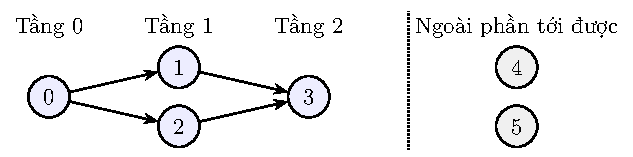
\includegraphics[width=\textwidth]{figures/bfs-example.pdf}
\caption[Ví dụ BFS sáu đỉnh]{BFS từ đỉnh $0$ trên đồ thị có hướng sáu đỉnh. Các cột biểu thị các tầng từ $0$ đến $2$ và các đỉnh ngoài phần tới được từ nguồn.}
\label{fig:bfs-example}
\end{figure}

\begin{table}[htbp]
\centering
\caption[Khoảng cách trong ví dụ BFS]{Khoảng cách và vị trí của sáu đỉnh trong Hình~\ref{fig:bfs-example}}
\label{tab:bfs-example}
\begin{tabular}{@{}lrrrrrr@{}}
\toprule
Đỉnh $v$ & 0 & 1 & 2 & 3 & 4 & 5 \\
\midrule
Khoảng cách $d[v]$ & 0 & 1 & 1 & 2 & $-1$ & $-1$ \\
Tập chứa đỉnh & $F_0$ & $F_1$ & $F_1$ & $F_2$ & \multicolumn{2}{c}{Ngoài phần tới được} \\
\bottomrule
\end{tabular}
\end{table}

Ở Hình~\ref{fig:bfs-example}, cả hai đỉnh $1$ và $2$ ở tầng $1$ đều có cung đến đỉnh $3$. Đỉnh $3$ chỉ xuất hiện một lần ở tầng $2$. Cả hai cung đều cho khoảng cách bằng $2$, nên thứ tự xử lý các đỉnh trong cùng tầng có thể thay đổi mà không làm đổi kết quả. Hai đỉnh cô lập $4$ và $5$ giữ giá trị $-1$ như trong Bảng~\ref{tab:bfs-example}.

\section{Biểu diễn CSR}
Dạng nén theo hàng (Compressed Sparse Row, CSR) lưu các đỉnh kề đi ra của mỗi đỉnh trong một đoạn liên tiếp \cite{barrett1994}. Nhóm dùng hai mảng:
\begin{itemize}
  \item \texttt{row\_offsets} có $n+1$ phần tử. Đoạn ứng với đỉnh $u$ bắt đầu tại \texttt{row\_offsets[u]} và kết thúc ngay trước \texttt{row\_offsets[u+1]}. Phần tử cuối bằng $m_{\mathrm{CSR}}$ và xác định điểm kết thúc của mảng cung.
  \item \texttt{col\_indices} có $m_{\mathrm{CSR}}$ phần tử. Mỗi phần tử là nhãn của một đỉnh đích.
\end{itemize}
Hai chỉ số bắt đầu liên tiếp bằng nhau khi đỉnh tương ứng không có cung đi ra. Với đồ thị không trọng số, CSR dùng cho BFS không cần mảng giá trị. Khi đồ thị đã được tạo, cả ba phiên bản chỉ đọc các mảng này. CSR giúp các phần tử liền kề của một hàng nằm sát nhau, còn thứ tự truy cập các hàng phụ thuộc vào thứ tự các đỉnh trong tập đỉnh biên.

\begin{figure}[htbp]
\centering
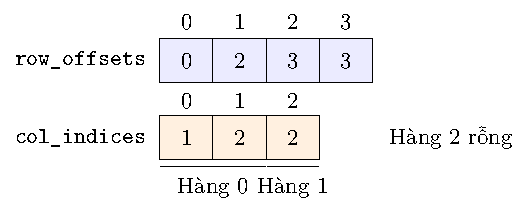
\includegraphics[width=.67\textwidth]{figures/csr-example.pdf}
\caption[Hai mảng CSR cho ba đỉnh]{Hai mảng CSR của đồ thị ba đỉnh với các cung $0\to1$, $0\to2$ và $1\to2$. Chỉ số mảng bắt đầu tại $0$.}
\label{fig:csr}
\end{figure}

Trong Hình~\ref{fig:csr}, đỉnh $0$ dùng đoạn $[0,2)$ của \texttt{col\_indices}, còn đỉnh $1$ dùng đoạn $[2,3)$. Hàng của đỉnh $2$ rỗng vì hai chỉ số giới hạn đều bằng $3$. Cạnh vô hướng giữa hai đỉnh khác nhau xuất hiện trong cả hai hàng tương ứng.

\section{OpenMP và các chính sách lập lịch}
OpenMP tạo nhóm luồng thực thi (thread team) trong vùng \texttt{parallel}, sau đó phân chia các vòng lặp bằng \texttt{omp for} \cite{trobec2018,openmp52}. Trong hai phiên bản của nhóm, một vùng song song phục vụ toàn bộ quá trình duyệt theo tầng. Công việc được chia theo chỉ số đỉnh trong frontier. Các đỉnh có thể có bậc ra khác nhau, nên hai luồng nhận cùng số đỉnh vẫn có thể phải xét số cung rất khác nhau.

Chính sách lập lịch (schedule) quyết định cách giao các lượt lặp. Với \texttt{static}, việc phân đoạn được xác định trước. Với \texttt{dynamic}, luồng nhận thêm đoạn khi hoàn thành đoạn trước. Với \texttt{guided}, kích thước đoạn giảm dần khi số lượt lặp chưa được cấp giảm. Hai chính sách cấp phát theo nhu cầu có thể hữu ích khi bậc ra chênh lệch, nhưng cần điều phối khi giao đoạn \cite{openmp52}. Mã hỗ trợ cả ba chính sách. Dữ liệu ở Chương~\ref{chap:experiment} dùng \texttt{static}.

Rào đồng bộ (barrier) buộc các luồng trong nhóm hoàn thành một pha trước khi chuyển sang pha phụ thuộc. Chỉ thị \texttt{omp for} và \texttt{single} trong hai cài đặt không có \texttt{nowait}, nên đều có rào ngầm ở cuối. Một vùng \texttt{single} cho đúng một luồng thực hiện công việc chung, chẳng hạn đổi hai tập đỉnh biên. Chỉ thị \texttt{omp barrier} tạo rào tường minh ở vị trí xuất hiện trong mã \cite{openmp52}.

\section{Chỉ số đánh giá hiệu năng}
\label{sec:metrics}
\subsection{Hệ số tăng tốc và hiệu suất}
Gọi $T_{\mathrm{Serial}}$ và $T_{\mathrm{OMP},p}$ lần lượt là trung vị thời gian của Serial và của một phiên bản OpenMP với $p$ luồng thực tế trên cùng đồ thị. Hai đại lượng báo cáo là
\[
 S_p=\frac{T_{\mathrm{Serial}}}{T_{\mathrm{OMP},p}},
 \qquad E_p=\frac{S_p}{p}.
\]
OpenMP có trung vị thấp hơn Serial khi $S_p>1$. Khi $S_p<1$, nghịch đảo $1/S_p$ cho biết OpenMP mất bao nhiêu lần thời gian của Serial. Bảng kết quả biểu diễn $E_8$ theo phần trăm. Đại lượng này chuẩn hóa tỷ số theo số luồng, nên không trực tiếp cho biết tỷ lệ CPU bận.

Khả năng mở rộng (scaling) cần so chính một cài đặt OpenMP ở nhiều số luồng trên cùng đầu vào. Chỉ số nội bộ $S_{\text{nội},p}=T_{\mathrm{OMP},1}/T_{\mathrm{OMP},p}$ giữ nguyên thuật toán. Chỉ số $S_p$ dùng Serial làm mốc để trả lời câu hỏi lựa chọn phiên bản. Thực nghiệm về khả năng mở rộng đo cả hai mốc trong cùng điều kiện; hiệu suất $E_p$ tính theo mốc Serial và đổi sang phần trăm bằng cách nhân $100$.

\subsection{Trung vị và tứ phân vị}
Với $N$ mẫu đã sắp tăng dần, đánh chỉ số từ $0$, vị trí của phân vị tại $q$ là $h=(N-1)q$. Nếu $i=\lfloor h\rfloor$ và $j=\lceil h\rceil$, giá trị phân vị là $x_i+(h-i)(x_j-x_i)$. Nhóm dùng $q=\num{0.25},\num{0.5},\num{0.75}$ để tính $Q_1$, trung vị và $Q_3$. Khoảng $[Q_1;Q_3]$ mô tả nửa giữa của phân bố theo các phân vị nội suy, còn độ rộng khoảng tứ phân vị (IQR) là $Q_3-Q_1$. Các đoạn sai số trong hình biểu thị khoảng này.

Khi thời gian Serial có độ phân tán lớn, nhóm thay tử số của $S_8$ lần lượt bằng $Q_1$ và $Q_3$ của Serial, giữ nguyên trung vị OpenMP. Phân tích này cho biết hệ số thay đổi thế nào khi dùng các phân vị khác nhau của thời gian Serial. Các tỷ số thu được mô tả độ nhạy theo mốc và không có diễn giải xác suất như khoảng tin cậy.

\subsection{Mô hình chi phí theo tầng}
Xấp xỉ $T_{\mathrm{OMP},p}\approx W/p+L\,t_{\text{tầng}}$ tách phần thời gian hữu ích trong điều kiện chia đều và chi phí phụ trội (overhead) lặp lại qua $L$ tầng. $W$ quy đổi lượng việc song song thành thời gian trên một luồng lý tưởng. $t_{\text{tầng}}$ biểu diễn một chi phí trung bình hiệu dụng, gộp điều phối, đồng bộ và thao tác chuẩn bị. Mô hình giúp hình thành giả thuyết cho đầu vào có nhiều tầng hẹp. Thời gian khởi tạo, chênh lệch lượng việc giữa các luồng và truy cập bộ nhớ có thể khiến xấp xỉ sai lệch. Tỷ số thời gian tổng chia cho số tầng vẫn chứa các thành phần này.

\section{Thiết kế và triển khai ba phiên bản}
\label{sec:implementations}
\subsection{Serial}
Serial dùng mảng hàng đợi FIFO với hai chỉ số đọc và ghi. Hàm khởi tạo toàn bộ $d$ bằng $-1$ và gán $d[s]=0$. Khi lấy đỉnh $u$ ở đầu hàng, hàm xét các cung đi ra và xếp vào cuối hàng mỗi đỉnh $v$ còn có $d[v]=-1$. Gán khoảng cách trước khi xếp hàng giúp mỗi đỉnh chỉ vào hàng đợi một lần. Thuật toán~\ref{alg:serial} mô tả trường hợp hàm hoàn tất phép duyệt.

\begin{algorithm}[htbp]
\caption{BFS tuần tự (Serial)}
\label{alg:serial}
\begin{algorithmic}[1]
\State Gán tất cả $d[v]\gets-1$, sau đó $d[s]\gets0$
\State Tạo hàng đợi FIFO $Q$ chứa $s$
\While{$Q$ còn phần tử}
  \State Lấy $u$ ở đầu $Q$
  \For{mỗi cung $(u,v)$ từ CSR}
    \If{$d[v]=-1$}
      \State $d[v]\gets d[u]+1$ và đưa $v$ vào cuối $Q$
    \EndIf
  \EndFor
\EndWhile
\State \Return $d$
\end{algorithmic}
\end{algorithm}

\subsection{Basic: bộ đếm nguyên tử dùng chung}
Hai bản OpenMP có hai mảng $F$ và $F'$ đủ sức chứa các đỉnh của một tầng. Ở Basic, một luồng đặt bộ đếm $c$ về $0$ trước khi cả nhóm mở rộng $F$. Khi thao tác nguyên tử trả về cờ cũ bằng $0$, luồng phát hiện $v$ lần đầu ghi $d[v]$ rồi gọi \texttt{atomic\_fetch\_add\_explicit} trên $c$. Giá trị trả về là chỉ số riêng để ghi $v$ vào $F'$. Cuối tầng, một luồng đọc số phần tử đã ghi và hoán đổi hai mảng. Thuật toán~\ref{alg:basic} thể hiện ba rào ngầm trong mỗi tầng được xử lý đầy đủ.

Nếu hai luồng cùng gặp đỉnh $3$ ở Hình~\ref{fig:bfs-example}, việc cùng đọc và ghi một cờ thường mà thiếu đồng bộ tạo ra tranh chấp dữ liệu (data race). Tình trạng tương tự xảy ra khi hai luồng cập nhật một bộ đếm thường và dùng chung chỉ số ghi. Đoạn rút gọn sau dựa trên \path{src/bfs_parallel_basic.c}, với bước truy cập hàng CSR và kiểm tra biên được lược bỏ. Đoạn này dùng thao tác nguyên tử C11 từ \texttt{<stdatomic.h>}. OpenMP phân việc và đồng bộ giữa các pha.
\begin{quote}\small\singlespacing
\begin{verbatim}
if (atomic_exchange_explicit(&visited[v], 1u,
                             memory_order_relaxed) == 0u) {
    distance[v] = distance[u] + 1;
    size_t j = atomic_fetch_add_explicit(next_size, 1u,
                                          memory_order_relaxed);
    next[j] = v;
}
\end{verbatim}
\end{quote}

\begin{algorithm}[htbp]
\caption{BFS OpenMP với bộ đếm chung (Basic)}
\label{alg:basic}
\begin{algorithmic}[1]
\State Mở một vùng \texttt{parallel}. Khởi tạo $d$ và \texttt{visited} bằng \texttt{omp for}
\State \texttt{single}: đặt nguồn vào $F$, đánh dấu nguồn và gán $d[s]=0$
\While{$F$ còn phần tử}
  \State \texttt{single}: đặt $c\gets0$ \Comment{Rào ngầm B1}
  \State \texttt{omp for}: chia các đỉnh $u\in F$ cho các luồng
  \For{mỗi cung $(u,v)$ của đỉnh $u$ đã được giao}
    \If{\Call{ExchangeRelaxed}{$\texttt{visited}[v],1$}$=0$}
      \State $d[v]\gets d[u]+1$
      \State $j\gets\Call{FetchAddRelaxed}{c,1}$ rồi ghi $F'[j]\gets v$
    \EndIf
  \EndFor
  \State Đóng \texttt{omp for} \Comment{Rào ngầm B2}
  \State \texttt{single}: đổi vai trò $F,F'$ và đặt kích thước $|F|\gets c$ \Comment{Rào ngầm B3}
\EndWhile
\end{algorithmic}
\end{algorithm}

\subsection{Optimized: ghép các bộ đệm riêng}
Ở Optimized, luồng $t$ ghi đỉnh mới vào bộ đệm riêng theo luồng (thread-local buffer) $L_t$ và đặt lại số phần tử khi bắt đầu tầng. Bộ đệm có thể tăng dung lượng và được tái sử dụng ở tầng sau. Khi vòng lặp duyệt kết thúc, một luồng tính chỉ số bắt đầu của từng đoạn ghi
\[
 o_0=0,\qquad o_t=\sum_{j=0}^{t-1}|L_j|,\qquad |F'|=o_p.
\]
Sau khi các chỉ số bắt đầu đã được xác định, mỗi luồng chép bộ đệm của mình vào đoạn $[o_t,o_{t+1})$ của $F'$. Một rào tường minh bảo đảm mọi đoạn đã được chép trước khi hoán đổi tập đỉnh biên. Thuật toán~\ref{alg:opt} sử dụng năm rào đồng bộ trong mỗi tầng được xử lý hoàn chỉnh.

\begin{algorithm}[htbp]
\caption{BFS OpenMP với bộ đệm theo luồng (Optimized)}
\label{alg:opt}
\begin{algorithmic}[1]
\State Mở một vùng \texttt{parallel}; chuẩn bị các bộ đệm và khởi tạo như Basic
\While{$F$ còn phần tử}
  \State Mỗi luồng $t$ đặt số phần tử của $L_t$ về $0$
  \State \texttt{single}: đặt lại cờ lỗi dùng chung \Comment{Rào ngầm O1}
  \State \texttt{omp for}: chia các đỉnh $u\in F$ cho các luồng
  \For{mỗi cung $(u,v)$ của đỉnh $u$ đã được giao}
    \If{\Call{ExchangeRelaxed}{$\texttt{visited}[v],1$}$=0$}
      \State $d[v]\gets d[u]+1$ rồi thêm $v$ vào $L_t$
    \EndIf
  \EndFor
  \State Đóng \texttt{omp for}, kiểm tra cờ lỗi \Comment{Rào ngầm O2}
  \State \texttt{single}: tính tổng tiền tố $o_0,\dots,o_p$ \Comment{Rào ngầm O3}
  \State Mỗi luồng $t$ chép $L_t$ vào $F'[o_t:o_{t+1})$
  \State \texttt{omp barrier} \Comment{Rào tường minh O4}
  \State \texttt{single}: đổi vai trò $F,F'$ và đặt $|F|\gets o_p$ \Comment{Rào ngầm O5}
\EndWhile
\end{algorithmic}
\end{algorithm}

\begin{figure}[htbp]
\centering
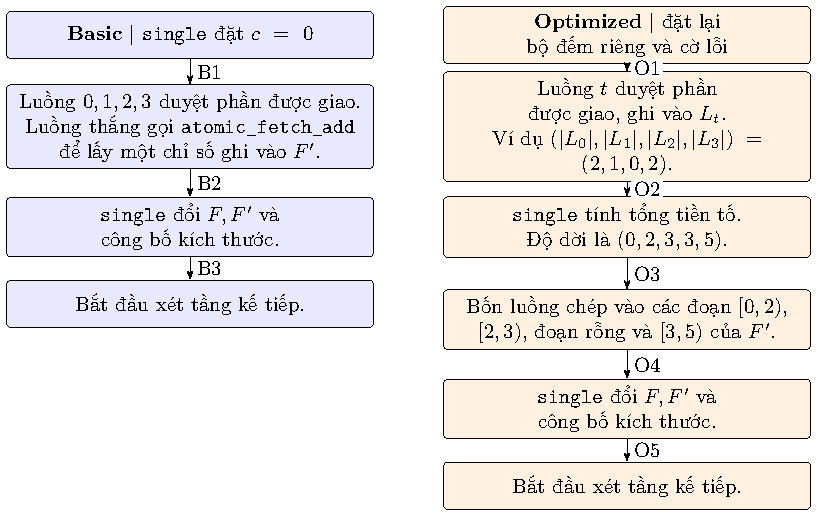
\includegraphics[width=\textwidth]{figures/frontier-design.pdf}
\caption[Một tầng của Basic và Optimized]{Các pha của một tầng thành công với bốn luồng. B1--B3 và O1--O5 là các rào đồng bộ. O4 là rào tường minh, các rào còn lại đều ngầm.}
\label{fig:design}
\end{figure}

Hình~\ref{fig:design} tách các pha phải hoàn tất trước khi chuyển sang pha kế tiếp. Basic cấp chỉ số ghi ngay khi phát hiện đỉnh mới. Optimized ghép các bộ đệm sau khi xác định số phần tử của từng luồng, do đó cần thêm hai rào đồng bộ. Bảng~\ref{tab:design} tóm tắt các thao tác làm nên sự khác biệt.

\begin{table}[htbp]
\centering
\caption[So sánh thiết kế OpenMP]{So sánh các thao tác khi xử lý một tầng}
\label{tab:design}
\begin{tabularx}{\textwidth}{@{}p{.27\textwidth}XX@{}}
\toprule
Thao tác & Basic & Optimized \\
\midrule
Xác nhận đỉnh mới & Cập nhật cờ nguyên tử & Cập nhật cờ nguyên tử \\
Ghi đỉnh mới & Ghi trực tiếp vào $F'$ & Ghi vào bộ đệm $L_t$ \\
Cấp vị trí ghi & Tăng bộ đếm chung & Tính tổng tiền tố \\
Hoàn tất $F'$ & Công bố kích thước & Chép các đoạn rồi công bố kích thước \\
Rào mỗi tầng & 3 rào ngầm & 4 rào ngầm, 1 rào tường minh \\
\bottomrule
\end{tabularx}
\end{table}

\section{Phân tích tính đúng đắn và chi phí}
\subsection{Bất biến và thứ tự bộ nhớ}
Tính nguyên tử của phép \texttt{atomic\_exchange\_explicit} bảo đảm chỉ một luồng nhận giá trị cờ cũ bằng $0$ và ghi $d[v]$. Thứ tự bộ nhớ \texttt{memory\_order\_relaxed} đủ cho việc xác nhận đỉnh mới vì sự đồng bộ giữa các pha được thực hiện bằng các rào OpenMP. Các luồng còn lại bỏ qua $v$ mà không đọc $d[v]$ trong tầng đó. Basic cấp chỉ số riêng bằng phép tăng nguyên tử. Optimized dùng các đoạn riêng xác định bằng tổng tiền tố.

Rào OpenMP bảo đảm việc ghi $d$ và tập đỉnh biên hoàn tất trước khi các luồng đọc dữ liệu ở pha sau. Hai cách tập hợp sinh cùng tập $F'$ theo lập luận ở Mục~\ref{sec:layers}. Bất biến về khoảng cách của các đỉnh trong $F$ vì thế được duy trì đến khi không còn tầng mới.

\subsection{Công việc và bộ nhớ}
Gọi $n_R$ và $m_R$ là số đỉnh tới được và số cung đi ra từ các đỉnh đó. Cả ba bản đều khởi tạo mảng khoảng cách kích thước $n$, xét mỗi đỉnh tới được một lần và duyệt đúng các cung đi ra từ chúng. Serial có công việc $O(n+m_R)$ và cần $O(n)$ bộ nhớ phụ. Basic cũng có công việc duyệt $O(n+m_R)$, với một phép đổi cờ trên mỗi cung được xét và một lần tăng bộ đếm trên mỗi đỉnh mới. Đếm thêm việc điều phối của $p$ luồng qua $L$ tầng cho một cận công việc theo mô hình $O(n+m_R+pL)$. Cận này không dự báo trực tiếp thời gian chờ tại rào hay khi nhiều luồng cùng truy cập biến nguyên tử.

Optimized thêm $O(pL)$ công việc tính tổng tiền tố và chép $n_R-1$ phần tử. Tăng dung lượng theo cấp số nhân cho chi phí thêm đỉnh khấu hao hằng số. Mỗi bộ đệm giữ dung lượng theo lần sử dụng lớn nhất của luồng. Tổng các cực đại không vượt $n_R-1$ vì mỗi đỉnh mới chỉ được ghi một lần. Hai mảng đỉnh biên, mảng đánh dấu, bộ đệm và bảng chỉ số dùng tổng cộng $O(n+p)$ bộ nhớ phụ.

